Nous avons vu que le problème du désassemblage tient dans la difficulté de séparer les parties de codes des parties de données d'un programme binaire.
Dans ce chapitre et dans un premier temps, nous proposons une preuve du caractère indécidable du désassemblage puis expliquerons les différentes techniques de désassemblage. Dans un second temps nous détaillerons notre approche du désassemblage qui permet de traiter le cas des programmes auto-modifiants ainsi que le chevauchement de code.


\paragraph{Difficulté théorique du désassemblage.}
~\\
\idone{Pb de l'arrêt: il existe HALT / pour tout P,I : HALT(P,I) = 1 ssi P(I) termine}
\itodo{Pb du désassemblage : borne min : intersection de CODE(P,I), borne max : union}
\itodo{borne min ~ arrêt ?}
% On a vu que le problème du désassemblage tient dans la difficulté de séparer les parties de code potentiel des parties de données.
Si on cherche à séparer le code des données alors le but du désassemblage d'un programme P est de résoudre le problème suivant. On se limite dans un premier temps à un programme P de taille finie et non auto-modifiant.
\begin{pb}
Soit \adr{a} une adresse, existe-t-il une entrée I de P telle que P(I) atteint \adr{a} ?
\end{pb}

Nous citons ici un argument tiré de la thèse de Joan Calvet \cite{Calvet2013} montrant le caractère indécidable de ce problème en réduisant le problème de l'arrêt à celui-ci.

% Supposons que le problème soit décidable. 
Notons CODE le programme vérifiant, pour tout programme P et adresse \adr{a}, CODE(P, \adr{a}) = 1 si et seulement si il existe une entrée I de P telle que P(I) atteint \adr{a}. Dans le cas contraire CODE (P, \adr{a}) = 0.

Soit P un programme ne prenant pas d'entrée et ayant un unique point d'arrêt indiqué par l'instruction \halt\ à l'adresse $\alpha$.
CODE(P, $\alpha$) = 1 si et seulement si P atteint l'adresse $\alpha$, c'est à dire si et seulement si P termine.
% . Prenons P' le programme suivant qui ne prend pas d'entrée : P' = P(I).

% Deux cas sont alors possibles.
% \begin{itemize}
%  \item Soit il existe une adresse $\alpha$ tel que l'instruction à l'adresse $\alpha$ est l'instruction d'arrêt \texttt{halt} et telle que CODE(P, $\alpha$) = 1 : il existe une entrée I' à P' telle que P'(I') atteint $\alpha$. Dans ce cas, puisque P'(I')=P'=P(I), P(I) atteint $\alpha$ et le programme P termine sur l'entrée I.
%  \item Dans le cas contraire il n'y a soit aucune instruction d'arrêt soit aucune de ces instructions n'est atteignable et donc P'(I')=P'=P(I) ne termine pas.
% \end{itemize}
% ~\\
Le désassemblage d'un programme dont le code est de taille infinie ou auto-modifiant est plus difficile que le cas traité ci-dessus et donc le résoudre permettrait également de traiter le problème de l'arrêt.
On en déduit donc que le désassemblage permet de résoudre le problème de l'arrêt qui est pourtant connu pour être indécidable ; c'est absurde.
Ainsi le problème du désassemblage est indécidable.


\paragraph{Analyse statique et dynamique.}
Dans le domaine de l'analyse de code, on parle d'analyse dynamique lorsque le fichier binaire à analyser est exécuté au moins partiellement et que l'analyse consiste à observer une ou des exécutions du programme. Au contraire lors d'une analyse statique on cherche à inférer des propriétés sur le programme sans l'exécuter.

Les deux techniques permettent de récupérer du code assembleur à partir du programme et donc de réaliser un désassemblage et de reconstruire un graphe de flot de contrôle.
L'avantage de l'analyseur dynamique est que, puisqu'il travaille sur une exécution spécifique du programme, il est précis : les instructions qui sont exécutées doivent être inclues dans le désassemblage.
Par contre il n'est pas complet vu qu'il ne suivra pas des branches du programme qui pourraient être utilisées si leurs conditions étaient vérifiées. À l'inverse un analyseur statique n'est pas précis et ne peut en général pas être complet à cause de l'impossibilité de prédire certaines cibles de sauts dynamiques.

En pratique le désassemblage est classiquement du domaine de l'analyse statique. Nous expliquerons comment l'analyse dynamique peut aider à reconstruire les graphes de flot et le code des programmes obscurcis.

\section{Désassemblage statique et chevauchement de code}
% \subsection{Couverture de code}
Nous cherchons à parcourir le plus de code atteignable et donc avoir une couverture optimale du code lors du désassemblage par rapport à un désassemblage parfait.
Il faut alors pallier à l'incomplétude d'un parcours récursif et au manque de précision d'un parcours linéaire.
Une des difficulté vient de l'obscurcissement par chevauchement de code. 
Nous cherchons donc des approches du désassemblage qui prennent en compte cette méthode de protection.
\\

Bien que le problème du chevauchement de code ne soit pas une technique d'obscurcissement récente et soit bien documenté \cite{PMA}, la littérature portant sur le désassemblage fait souvent l'hypothèse qu'un octet à une adresse spécifique ne peut être présent que dans une seule instruction \cite{KruegelRVV04}. Cette contrainte empêche de détecter tout chevauchement mais permet un désassemblage plus précis sur un binaire qui n'utilise pas cette technique de protection.



Les auteurs de la technique de chevauchement détaillée au chapitre \ref{chap:obscurcissement}, permettant d'encoder une séquence de code cachée dans une séquence \cite{JLH13}, proposent de détecter la protection qu'ils exposent. L'idée est qu'il est improbable qu'une longue séquence d'octets représente une séquence valide de code. Si une telle séquence existe, c'est sûrement du code caché. Cette approche fonctionne pour la protection qu'ils exposent mais n'est pas applicable aux cas de \telock\ ou UPX par exemple car les séquences d'octets sur lesquels des instructions se chevauchent sont très courtes.

\paragraph{Désassembleurs disponibles.}
Les désassembleurs existants, qu'ils utilisent un parcours linéaire ou récursif, font l'hypothèse que le code ne peut pas se chevaucher et ne parviennent pas à afficher un désassemblage cohérent dans le cas contraire.

Le désassemblage récursif de l'exemple de \telock\ avec IDA Pro (version 6.3) \cite{IDA} est le suivant :
\begin{lstlisting}[language={[x86masm]Assembler}, escapechar=~]
01006E7A     inc     byte ptr [ebx+ecx]
01006E7D     jmp     short near ptr loc_1006E7D+1
; ~Les octets qui suivent n'ont pas été désassemblés~
01006E7F     db 0C9h
01006E80     db  7Fh
01006E81     db 0E6h
01006E82     db  8Bh
01006E83     db 0C1h
\end{lstlisting}
Radare \cite{radare} effectue le désassemblage linéaire suivant :
\begin{lstlisting}[language={[x86masm]Assembler}, escapechar=~]
01006e7a    fe 04 0b     inc byte [ebx+ecx]
01006e7d    eb ff        jmp 6e7e
01006e7f    c9           leave
01006e80    7f e6        jg 6e68
01006e82    8b c1        mov eax, ecx
\end{lstlisting}
Ni l'un ni l'autre n'est capable de suivre le saut de l'instruction \jmp\ : la cible du saut a déjà été prise en compte comme faisant partie d'une autre instruction.

De même ni Radare ni IDA ne détectent le second chemin d'exécution dans l'extrait d'UPX et désassemblent cet extrait comme suit.
\begin{lstlisting}[language={[x86masm]Assembler}, escapechar=~]
010059f0    89 f9            mov ecx, edi
010059f2    79 07            jns 0x10059fb
010059f4    0f b7 07         movzx eax, word [edi]
010059f7    47               inc edi
010059f8    50               push eax
010059f9    47               inc edi
010059fa    b9 57 48 f2 ae   mov ecx, 0xaef24857
010059ff    55               push ebp
\end{lstlisting}

\paragraph{Parcours spéculatif.}
Le parcours récursif étant moins sensible à des obscurcissements très simples comme l'injection de code mort, il est souvent pris comme point de départ dans les recherches sur le désassemblage statique.
Une fois une première recherche de code avec un parcours récursif effectuée, les octets restants peuvent subis un parcours linéaire qui cherchera à déterminer s'ils sont du code ou des données à l'aide d'heuristiques.
Une de ces approche évalue la probabilité qu'une suite d'octets soit effectivement du code en apprenant au préalable des suites d'octets codant réellement des instructions lancées lors de l'exécution de programmes \cite{KDF09}.
On appelle cet enchaînement des deux parcours un parcours spéculatif.

Prasaf et Chiueh \cite{PC03}, après un premier désassemblage récursif, tentent d'identifier les adresses de début de fonctions assembleur à l'aide de la suite d'instruction \push\ puis \mov, caractéristique de fonctions compilées : elles commencent par empiler le pointeur de pile de base avec \texttt{push ebp} pour le remplacer par le pointeur de pile avec \texttt{mov ebp, esp}. Ils identifient également toutes les adresses où sont codées une instruction valide. À partir de ces adresses ils effectuent à nouveau un parcours récursif. Le risque est alors grand que des chemins parcourus ainsi soient invalident, ils éliminent les chemins qui n'aboutissent ni sur un \ret\ ni sur un \jmp\ puisqu'ils aboutissent du coup sur des données.

% \paragraph{Dans la littérature.}

% \\



% \paragraph{Chevauchement de code.}
Krügel, Roberston, Valeur et Vigna \cite{KruegelRVV04} proposent aussi de séparer le code en fonctions assembleur. Ils effectuent une première analyse récursive pour détecter le maximum d'instructions atteignables et, lorsque que deux ou plusieurs instructions atteignables se chevauchent, ils considèrent qu'il s'agit d'un conflit qui se résoudra par le choix d'une des instructions.
Leurs hypothèses sont : (i) les instructions ne peuvent pas se chevaucher, (ii) les sauts conditionnels peuvent être suivis ou non, (iii) le binaire peut contenir du code mort, et (iv) le code suivant une instruction \call\ n'est pas nécessairement accessible. Pour résoudre les conflits de chevauchement ils favorisent les instructions atteignables depuis le point d'entrée (que l'on sait accessible), puis ils considèrent qu'une instruction permettant d'atteindre directement deux instructions qui se chevauchent n'est pas valide et enfin ils favorisent les instructions les plus connectées au graphe de flot de contrôle.
Leur approche est un point de départ pour le désassemble de binaires obscurcis. Ils prennent par exemple en compte l'ajout de code mort et certaines modifications du flot de contrôle.

Schwarz, Debray et Andrews \cite{SDA02} introduisent un parcours linéaire capable de détecter certaines injections de données dans le code, comme les tables de saut (souvent présent dans du code compilé en C ou C++). Ils proposent de combiner les parcours récursifs et linéaires pour détecter les anomalies dans le désassemblage. Si, au sein d'une fonction, une instruction provenant du désassemblage récursif chevauche une instruction provenant du désassemblage linéaire, le désassemblage de la fonction est considéré comme contenant une erreur.
\\

Partant du principe qu'un désassemblage correct ne contient pas de chevauchement de code, ces approches ne sont pas satisfaisante pour désassembler des binaires utilisant du chevauchement de code, tels les programmes protégés avec \telock.
\\

Dans sa thèse, Kinder \cite{Kinder10} indique que si la technique de désassemblage ne prend pas de contrainte de d'alignement du code et réalise des désassemblages atomiques d'une seule instruction à la fois à partir de chaque adresse, alors on peut voir deux instructions qui se chevauchent comme indépendantes. Effectivement les travaux présentés dans cet état de l'art ainsi que les désassembleurs existants prennent pour hypothèse que le code ne doit pas se chevaucher alors que nous avons représenté les chevauchements de \telock\ et UPX très simplement. L'hypothèse d'alignement permet en général de simplifier les critères de désassemblage et est justifiée par la non occurrence de ce phénomène dans des programmes légitimes.
Nous verrons qu'en pratique l'utilisation du chevauchement de code est rare même dans un binaire protégé et nous proposerons une technique de désassemblage capable de détecter les cas de chevauchement.


\section{Analyse dynamique et auto-modification}
L'analyse dynamique consiste à se baser sur une ou des exécutions particulières d'un programme pour inférer des propriétés sur son fonctionnement.
Elle demande donc de se munir d'une langage modélisant le fonctionnement de la machine durant l'exécution du programme, d'une sémantique concrète de l'assembleur utilisé et de lancer l'évaluation sémantique du programme sur une ou plusieurs entrées.
Les entrées d'un programme sont par exemple les paramètres passés lors de l'appel au programme, l'état de la machine lors du démarrage, les données lues depuis la mémoire et les saisies faites par l'utilisateur au clavier ou à la souris lors de l'exécution s'il s'agit d'une application dotée d'une interface graphique.

Dans cette partie nous reprendrons la sémantique simplifiée pour un langage assembleur définie au chapitre précédent et expliquerons comment séparer une exécution d'un programme auto-modifiant en plusieurs sous-exécution non auto-modifiantes afin d'utiliser des techniques standard d'analyse sur chacune de ces sous-exécutions.



\subsection{Auto-modification et vagues}
Si on reprend l'exemple de code auto-modifiant du chapitre précédent (figure \ref{fig:unevague_v0}), on peut construire trois représentations en mémoire des parties exécutables du programme.
La première correspond à la vision du programme lors de son chargement : la section .text est dans son état initial.
La seconde est celle après que la première modification du programme faite à l'adresse \adr{8048086} et la troisième après la seconde modification faite à l'adresse \adr{804808b}.
En fait vu qu'aucune des adresses modifiées par la première instruction auto-modifiante n'est exécutées avant que la seconde modification ne soit faite, on peut regrouper les deux instructions auto-modifiantes et considérer que le programme n'a que deux représentations en mémoire : la représentation initiale et la représentation au moment où l'instruction modifiée à l'adresse \adr{8048091} est exécutée.

Dans ce découpage informel on appelle vague une représentation mémoire à un instant donné. 
L'exécution d'un programme est alors caractérisée par une suite d'exécutions sur des vagues successives comme représenté en figure \ref{fig:vagues_visuel}. Les instructions qui sont présentes dans la trace sont colorées en rose tandis que le point d'entrée et la dernière instruction sont en orange et bleu clair, respectivement.
On passe d'une vague $k$ à la vague suivante $k+1$ lorsqu'une adresse mémoire écrite dans la vague $k$ est exécutée.
Ainsi dans une vague $k$, toutes les instructions exécutées ont été écrites au moins à la vague $k-1$. 
En ce sens chacune des vagues, prise indépendamment des autres, ne présente pas d'auto-modification.

Nous détaillerons par la suite ce qu'est une trace d'exécution pour l'analyse dynamique ainsi que la sémantique d'enchaînement des vagues.

\begin{figure}
 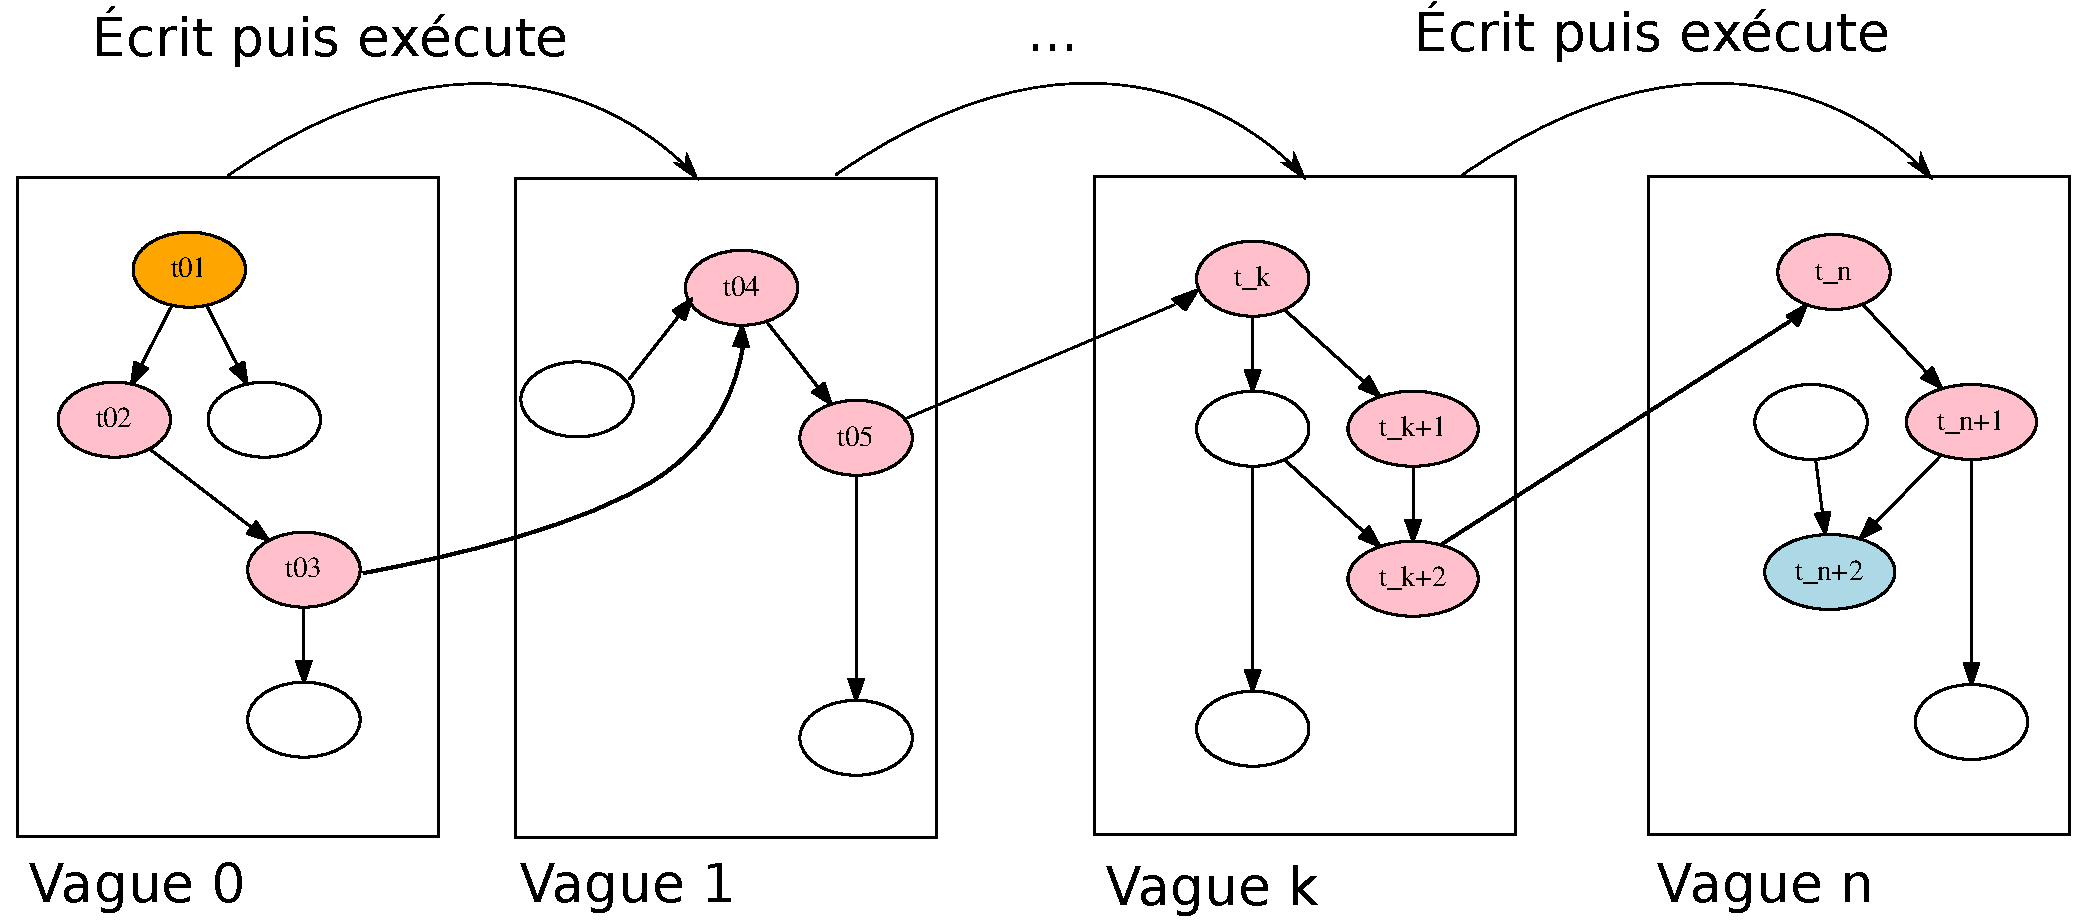
\includegraphics[width=1.0\textwidth]{supports/automodification/phases2_final.pdf}
 \caption{Vision informelle des vagues}
 \label{fig:vagues_visuel}
\end{figure}


\subsection{Revue de littérature}
La notion de vague présentée dans ce chapitre a été développée dans les thèse de Reynaud \cite{Reynaud2010} et Calvet \cite{Calvet2013}.
Elle est similaire à la notion de \emph{phase} présentée par Debray et Patel \cite{DP10} et utilisée pour automatiser la suppression de la protection d'un binaire. Le découpage d'une trace en phases est, chez eux, identique au découpage en vagues que l'on présent dans ce chapitre.
En général la suppression des protections se fait à l'aide d'une analyse dynamique et d'une image de la mémoire à un instant donné au cours de l'exécution. C'est cette image mémoire qui sera considéré comme était le programme d'origine. La difficulté réside alors dans le choix de l'instant où prendre l'image mémoire.

Preda, Giacobazzi, Debray, Coogan et Townsend \cite{PGDCT10} utilisent la même notion de phases mais chaque lecture d'une instruction écrite lors d'une vague précédente (pas uniquement lors de la phase en cours) provoque la création d'une nouvelle phase.


\subsection{Trace, niveaux d'exécution et vagues}
Le programme exécuté a pour sources principales de données les registres et la mémoire constituée de la pile et du tas qui sont tous les deux adressables par des entiers. Une variable d'un programme est donc soit un registre du processeur soit une adresse mémoire, de même que défini dans la sémantique du langage intermédiaire défini au chapitre précédent (définition \ref{def:sem_conc_var}).

En utilisant la sémantique concrète précédemment définie on est capable, à partir d'un ensemble de valeurs initiales pour les registres et la mémoire, d'exécuter un programme sur cette entrée.
Une trace d'exécution d'un programme est simplement l'enchaînement des instructions auxquelles l'exécution du programme a fait appel. Si on note $I_i$ une instruction dynamique, la trace d'exécution est $T=I_1, I_2, ..., I_n$ où $I_n$ est la dernière instruction du programme.

Nous définissons une instruction dynamique (définition \ref{def:ensembles_inst_dyn}) par son adresse, les adresses mémoires sur lesquelles elle est codée et l'instruction machine correspondant. Ces informations sont données par un désassemblage atomique d'une instruction à l'adresse mémoire spécifiée.
Afin de pouvoir séparer la trace d'exécution selon le moment où chaque instruction a été écrite, nous définissons aussi pour chaque instruction l'ensemble des variables sur lesquelles elle provoque une écriture. Cette information est donnée par la sémantique concrète choisie. Avec la sémantique définie à la section précédente les seules instructions qui provoquent des écritures sont celles dont la liste d'instructions atomiques donnée par le désassemblage contiennent des assignation de la forme $x\leftarrow g(x_1, ..., x_m)$ : \dw{D}=\dw{d_1..d_n}=\dw{d_1}$\ \cup\ ...\ \cup\ $\dw{d_n} avec
\\
\dw{d_i}$=
\left\{
  \begin{array}{ll}
	  x &$ si $d_i=x\leftarrow g(x_1, ..., x_m)\ et\ x\in\BV
	\\\Theta(v) &$ si $d_i=x\leftarrow g(x_1, ..., x_m)\ et\ x\notin\BV$: $x=[v]$ avec $v\in\BV
	\\ \emptyset &$ sinon.$
  \end{array}
\right.
$

\begin{defi}
On note $D$ une instruction dynamique constituée des éléments suivants.
\begin{itemize}
 \item \da{D} l'adresse mémoire de l'instruction dynamique
 \item \dc{D} le segment des adresses mémoire sur lequel \di{D} est codée
 \item \di{D} l'instruction machine à l'adresse \da{D}
%  \item \dr{D_i} l'ensemble des variables sur lesquelles l'exécution de \di{D_i} provoque une lecture
 \item \dw{D} l'ensemble des variables sur lesquelles l'exécution de \di{D} provoque une écriture
\end{itemize}
\label{def:ensembles_inst_dyn}
\end{defi}

Nous avons donc, pour une trace d'exécution donnée, des vagues successives $1, 2, ..., n$.
Au cours de l'exécution du programme on définit, pour chaque adresse en mémoire $m$, un niveau d'écriture $W^M[m]$.
correspondant à la dernière vague $k$ durant laquelle une instruction a modifié la valeur à l'adresse $m$.


Une instruction $D$ a un niveau d'exécution $X$, comme indiqué en définition \ref{def:write_exec_levels}.
Elle a également a un niveau d'écriture $W_D$ qui est le niveau d'écriture le plus élevé parmi les adresses sur lesquelles elle est codée : $W_D=max(W^M[a],\ a\in\ $\dc{D_i}$)$.


\begin{defi}
Nous définissons une trace d'exécution comme la donnée d'une suite $T=t_1, t_2, ..., t_n$ composée de triplets de la forme $t_i=(i, D_i, X_i)$ tels que
\begin{itemize}
 \item $D_i$ est la $i^{eme}$ instruction dynamique exécutée.
 \item Avant l'exécution de l'instruction $D_i$, le niveau d'exécution est \texttt{$X_{i-1}$}.
 \item Après l'exécution de l'instruction $D_i$, le niveau d'exécution est \texttt{$X_i$}.
\end{itemize}
\label{def:write_exec_levels}
\end{defi}

\begin{propri}
 Si le niveau d'exécution courant est $X$, le niveau d'exécution de l'instruction à exécuter $D_i$ est :\\
 $X=max(X, W_D+1)$ avec $W_D=max(W^M[a],\ a\in\ $\dc{D_i}$)$.\\
 Après l'exécution de $D_i$, les niveaux d'écriture dans la mémoire sont mis à jour de la manière suivante :\\
 $\forall a\in$ \dw{D_i}, $W^M[a]=X$.
\label{propri:niveau_exec}
\end{propri}

En pratique une instruction $D$ écrite par une instruction ayant pour niveau d'exécution $k$ puis directement exécutée aura pour niveau d'écriture $W_D=k$ et pour niveau d'exécution $X=k+1$. Ce comportement est formalisé par la propriété \ref{propri:niveau_exec}.

On définit alors formellement la vague $k$ selon la définition \ref{def:vagues} et l'algorithme \ref{algo:analyse_dyn_vagues} permet d'exécuter un programme dynamiquement avec la sémantique concrète choisie tout en déterminant les niveaux d'exécution de d'écriture au fur et à mesure de l'exécution. La sortie de l'algorithme \ref{algo:analyse_dyn_vagues} est la trace d'exécution et la liste des vagues reconstruites.
\\

Reprenons l'exemple du programme auto-modifiant de la figure \ref{fig:unevague_trace}.
La figure \ref{fig:unevague_trace} donne une trace d'exécution de ce programme en détaillant les informations sur chaque instruction dynamique ainsi que les niveaux d'écriture et d'exécution de chaque instruction.
Au départ toute la mémoire est dans son état d'origine et a pour niveau d'exécution 0. Lorsque l'instruction $D_0$ est exécutée, il n'y a pas eu d'auto-modification donc le niveau d'écriture est 0 et le niveau d'exécution est 1.
Les instructions $D_3$ et $D_4$ provoquent une auto-modification : les octets aux adresses \adr{0x8048091} et \adr{0x8048092} sont modifiés et leurs niveaux d'écriture deviennent donc le niveau d'exécution courant, soit 1.
Lorsque l'exécution atteint $D_5$, qui a été modifié, le niveau d'écriture est 1 donc le niveau d'exécution devient 2.
L'instruction suivante $D_6$ fixe la valeur de \edi\ à 2 puis les instructions suivantes provoquent l'affichage de \edi.

Cette trace d'exécution est donc composée de deux vagues : la vague initiale, $v_0$ composée de l'état de la mémoire avant l'exécution de la première instruction et la vague $v_1$ contenant l'état de la mémoire juste après l'exécution de $D_4$ et avant l'exécution de la première instruction modifiée $D_5$.




\begin{defi}
 Étant donné une trace d'exécution $T=t_1, ..., t_n$ avec $t_i=(i, D_i, X_i)$ et $k\in\{X_j, 1\leq i\leq n\}$, on appelle vague $k$ l'état de la mémoire juste après l'exécution de la dernière instruction ayant pour niveau d'exécution $k$.
 C'est à dire l'état de la mémoire juste après l'instruction $D_j$ avec $X_{j+1}>k$.
 \label{def:vagues}
\end{defi}

% \begin{algorithm}[H] %or another one check
% \caption{Mise à jour des niveaux d'exécution et d'écriture lors de l'exécution d'une instruction}
% \SetAlgoLined
% \KwIn{La mémoire, l'opérateur de niveau d'écriture, une instruction dynamique et le niveau d'exécution courant}
% \KwResult{L'opérateur de niveau d'écriture et le niveau d'exécution courant mis à jour}
% \SetKwProg{Fn}{}{}{}
% \SetKwFunction{FRecurs}{calculNiveau}
% \Fn(
% ){\FRecurs{M, $W^M$, D, X}}{
% $W_D \leftarrow\ max(W^M[a],\ a\in\ $\dc{D}$)$\\
% $X \leftarrow\ max(X,\ W_D+1)$ \\
% \For {$m\in\ $\dw{D}}{
%   $W^M[m]\leftarrow\ X$
% }
% \Return ($W^M$, X)
% }
% \label{algo:update_vagues}
% \end{algorithm}

\begin{algorithm}[H] %or another one check
\caption{Mise à jour du niveau d'exécution d'une instruction}
\SetAlgoLined
\KwIn{La mémoire, l'opérateur de niveau d'écriture, une instruction dynamique et le niveau d'exécution courant}
\KwResult{Le niveau d'exécution courant mis à jour}
\SetKwProg{Fn}{}{}{}
\SetKwFunction{FRecurs}{MAJExecution}
\Fn(
){\FRecurs{M, $W^M$, D, X}}{
$W_D \leftarrow\ max(W^M[a],\ a\in\ $\dc{D}$)$\\
$X \leftarrow\ max(X,\ W_D+1)$ \\
\Return X
}
\label{algo:update_exec_level}
\end{algorithm}

\begin{algorithm}[H] %or another one check
\caption{Mise à jour des niveaux d'écriture lors de l'exécution d'une instruction}
\SetAlgoLined
\KwIn{La mémoire, l'opérateur de niveau d'écriture, une instruction dynamique et le niveau d'exécution courant}
\KwResult{L'opérateur de niveau d'écriture mis à jour}
\SetKwProg{Fn}{}{}{}
\SetKwFunction{FRecurs}{MAJEcriture}
\Fn(
){\FRecurs{M, $W^M$, D, X}}{
\For {$m\in\ $\dw{D}}{
  $W^M[m]\leftarrow\ X$
}
\Return $W^M$
}
\label{algo:update_write_level}
\end{algorithm}

\begin{figure}
\begin{center}
\begin{tabular}[b]{|l|l|l|l|l|l|l|}
\hline
i & \da{D_i} & \dc{D_i} & \di{D_i} & \dw{D_i} & $W_i$ & $X_i$ \\
\hline
& 8048060  &  (...)         	        & Pile -> RWX &  & 0 & 1 \\ 
1 & 804807c  &  [804807c, 8048080]         &  mov    edi, 0x0 & edi & 0 & 1 \\
2 & 8048081  &  [8048081, 8048086]         &  mov    eax, 0x8048091 & eax & 0 & 1 \\
3 & 8048086  &  [8048086, 804808a]         &  mov    [eax], 0xeb & 0x8048091 & 0 & 1 \\
4 & 804808b  &  [804808b, 8048090]         &  mov    [eax+1], 0x7 & 0x8048092 & 0 & 1 \\
5 & 8048091  &  [8048091, 8048092]         &  jmp    80480a1 <edi3> &  & 1 & 2  \\
6 & 804809a  &  [804809a, 804809d]         &  mov    edi,0x2 & edi & 0 & 2\\
7 & 804809f  &  [804809f, 80480a0]         &  jmp    80480a8 <fin> &  & 0 & 2\\
 & 80480a8  &  (...)		        &  Affiche edi &  & 0 & 2\\
 & 80480c3  &  (...)		        &  Quitte &  & 0 & 2\\
\hline
\end{tabular}
\end{center}
\caption{Trace d'exécution du programme auto-modifiant de la figure \ref{fig:unevague_v0}}
\label{fig:unevague_trace}
\end{figure}

\begin{algorithm}[H] %or another one check
\caption{Analyse dynamique avec calcul des vagues}
\SetAlgoLined
\KwIn{Les registres R et une mémoire M dans laquelle un programme a été chargé à son point d'entrée \texttt{ep}}
\KwResult{La trace des instructions dynamiques chacune associée à leur niveau d'exécution et les différentes vagues de la trace}
\SetKwProg{Fn}{}{}{}
\SetKwFunction{FRecurs}{analyseDynamique}
\Fn(
% \tcc*[h]{C : matrice des associations possibles, i : numéro du prochain sommet de P à associer, F : liste des couples d'associations déjà faites}
){\FRecurs{R, M, ep}}{
\For{$m\in M$}{
  $W^M[m]\leftarrow 0$\\
}
$X\leftarrow 1$\\
$X_{-1}\leftarrow 0$\\
$i\leftarrow 0$\\
$T\leftarrow \emptyset$\\
$vagues\leftarrow \emptyset$\\
$eip\leftarrow ep$\\
\While {la fin du programme n'est pas atteinte} {
$i\leftarrow i+1$\\
~\\
$D\leftarrow decode(eip, M)$\\
$X\leftarrow MAJExecution(M, W^M, D, X)$\\
\If {$X \ne X_{-1}$}{
  $vagues\leftarrow vagues\cup \{(X_{-1}, M)\}$
}
$X_{-1} \leftarrow X$\\
~\\
$(eip, R, M)\leftarrow sem\_eval(eip, R, M)$\\
$W^M\leftarrow MAJEcriture(M, W^M, D, X)$\\
$T\leftarrow T\cup\{(i, D_i, X)\}$\\
}
\Return T, vagues
}
\label{algo:analyse_dyn_vagues}
\end{algorithm}

\begin{rem}
 Étant donné la définition croissante des vagues, la même instruction $D$ peut-être exécutée non seulement plusieurs fois dans la même vague mais également être présente à des vagues différentes.
\end{rem}

\subsection{Implémentations}
\todo[inline]{émulation VS instrumentation VS déboguage}
\todo[inline]{BAP: \\
Jakstab: \\
TraceSurfer: (outil de daniel)\\
Renovo : \\
LLVM : (pk ne pas l'utiliser??) \\
Implem en C: \\
Pin : \\
Xed : \\
}

Plusieurs choix s'offrent à qui cherche à implémenter un système d'analyse dynamique de binaire.


% \subsection{Revue de littérature}
\subsection{Émulation avec BAP}
\subsection{Instrumentation avec Pin}


\section{Analyse statique et chevauchement de code}
Nous cherchons à formaliser le problème du chevauchement de code.
Du point de vue du désassemblage, un programme qui présente une unique instruction qui en chevauche une autre peut se voir comme composé d'un chemin principal de désassemblage et d'un chemin secondaire dans lequel l'instruction en chevauchement se place.
Reprenons l'exemple de \telock : le segment d'octets \texttt{eb ff c9 7f e6} peut se voir comme composé des deux \layers\ de code données à la figure \ref{fig:telock-layers-simple} : il y a deux \layers, la première contient les instructions \texttt{jmp +1}, \texttt{leave} et \texttt{jg 0x1006e68} et la seconde contient l'instruction \texttt{dec ecx}, chevauchant \texttt{jmp +1}.
En fait le segment d'octets \texttt{eb ff c9 7f e6} contient exactement les quatre instructions précédentes : il y a au maximum une instruction valide à chaque adresse et la dernière instruction potentielle, codée sur \texttt{e6}, n'est pas valide.


\begin{figure}
\begin{center}
\begin{tabular}{|l|c|c|c|c|c|}
\hline
Adresses & 0x01006e7d & 0x01006e7e & 0x01006e7f & 0x01006e80 & 0x01006e81\\
\hline
Octets & eb & ff & c9 & 7f & e6\\
\hline
\Layer\ 1 & \multicolumn{2}{c|}{jmp +1} & leave & \multicolumn{2}{c|}{jg 0x1006e68}\\
\hline
\Layer\ 2 & \cnoir & \multicolumn{2}{c|}{dec ecx} & \multicolumn{2}{c|}{\cnoir} \\
 \hline
% \\
\end{tabular}
\end{center}
\caption{Découpage cohérent en \layers\ de l'extrait de \telock}
\label{fig:telock-layers-simple}
\end{figure}

% \begin{figure}
% \begin{center}
% \begin{tabular}{|l|c|c|c|c|c|}
% \hline
% Adresses & 0x01006e7d & 0x01006e7e & 0x01006e7f & 0x01006e80 & 0x01006e81\\
% \hline
% Octets & eb & ff & c9 & 7f & e6\\
% \hline
% \Layer\ 1 & \multicolumn{2}{c|}{jmp +1} & \cnoir & \multicolumn{2}{c|}{jg 0x1006e68}\\
% \hline
% \Layer\ 2 & \cnoir & \multicolumn{2}{c|}{dec ecx} & \multicolumn{2}{c|}{\cnoir} \\
%  \hline
% % \\
% \end{tabular}
% \end{center}
% \caption{\Layers\ de l'extrait de \telock}
% \label{fig:telock-layers-recursive}
% \end{figure}

Formellement on définit une \layer\ comme un ensemble d'instructions qui ne se chevauchent pas (définition \ref{def:layer}).
Par conséquent lors du désassemblage on cherche à effectuer un découpage cohérent des instructions inclues dans le graphe de flot de contrôle en différentes \layers. Un découpage cohérent est simplement la donnée d'un ensemble de \layers\ deux à deux disjointes et recouvrant l'ensemble des instructions désassemblées.
L'exemple précédent pour \telock\ est un découpage cohérent.

\begin{defi}
 Une \layer\ de code $L$ est un ensemble d'instructions dynamiques qui ne se chevauchent pas : $\forall D_1, D_2\in L,\ $\dc{D_1}$\cap$\dc{D_2}$=\emptyset$.
\label{def:layer}
\end{defi}

\paragraph{Borne du nombre de \layers.}
Le nombre minimal de \layers\ permettant de former un découpage cohérent est borné par la taille maximale des instructions, c'est à dire 15 octets pour l'assembleur \xq.
Pour s'en convaincre il suffit de définir le découpage cohérent suivant. Pour un segment d'octets à l'adresse \adr{a}, on place dans la \layer\ i, pour $1\leq i\leq 15$ toutes les instructions aux adresses congrues à $a+i-1 (mod\ 15)$. C'est à dire que la \layer\ 1 contient les instructions aux adresses \adr{a}, \adr{a+15}, \adr{a+30}, etc ; la \layer\ 2 celles aux adresses \adr{a+1}, \adr{a+16}, \adr{a+31}, etc. Puisque les instructions dans chaque \layer\ sont distantes de 15 octets, il ne peut pas y avoir de chevauchement au sein d'une \layer\ et les \layers\ sont disjointes ; il s'agit bien d'un découpage cohérent une fois qu'on enlève les \layers\ ne contenant pas d'instructions valides. Ce découpage contient au plus 15 \layers.
\itodo{l'exemple qui donne 15 layers ?}

Nous définirons par la suite plusieurs découpages cohérents en \layers\ et discuterons de leur pertinence et de leurs implémentations.


\subsection{\Layers\ linéaires}
Une approche naturelle des \layers\ consiste à construire une première \layer\ par parcours linéaire à partir du début de la section de code du binaire.
Cette première \layer\ contient exactement les instructions qu'un désassembleur par parcours linéaire aurait détecté.
Les \layers\ suivantes seront construites également par parcours linéaire, à partir de chaque adresse du binaire.
Ainsi on peut construire une \layer\ de code à partir de chaque adresse du binaire.
Un tel découpage pour \telock\ donne les layers indiqués en figure \ref{fig:telock-layers-linear}.

Ce découpage est donc, par définition, basé sur l'alignement des instructions : au sein d'une \layer, les instructions sont alignées, c'est à dire qu'un désassemblage linéaire depuis la première instruction de la \layer\ parcourt toutes les autres instructions de la \layer. 
Il est à noter qu'en assembleur \xq\ ou \xs\ les instructions ont tendance à se réaligner rapidement : si deux instructions se chevauchent et qu'on l'on réalise un parcours linéaire depuis chacune d'entre elles, il suffit en général d'au plus quatre \todo{cite, vrai?}instructions pour que ces deux parcours se confondent.
Cette propriété a pour conséquence que la plupart des \layers\ linéaires se réalignent sur une \layer\ précédente, en général la première. Sur la figure \ref{fig:telock-layers-linear} les \layers\ 1 et 2 se réalignent et partagent l'instruction \texttt{jg 0x1006e68}.
Cette propriété n'est évidemment pas vérifiée si les instructions ont été spécialement choisie pour provoquer de longs chemins de chevauchement, comme avec l'obscurcissement précédemment cité \cite{JLH13}.

Nous souhaitons obtenir un découpage cohérent des \layers\ sous forme d'ensembles deux à deux disjoints.
Il suffit alors d'enlever des \layers\ les instructions existant déjà dans les \layers\ inférieures (colorées en gris sur la figure \ref{fig:telock-layers-linear}) et de ne garder que les \layers\ contenant des instructions valides.
Au final il reste les deux \layers\ données précédemment à la figure \ref{fig:telock-layers-simple}, obtenus linéairement.

\paragraph{Binaire composé de plusieurs segments.}
On peut étendre la définition précédente applicable à un segment d'octets à un binaire composé de plusieurs segments de code disjoints.
L'extension consiste à simplement à réaliser un découpage cohérent pour chaque segment puis à les réunir au sein d'un seul découpage par une union des \layers\ qui les composent, lui aussi cohérent puisque les segments sont deux à deux disjoints.

\paragraph{\Layers\ linéaires et désassemblage.}
% Les \layers\ linéaires sont en fait une extension du désassemblage linéaire. Un programme non obscurcis peut être désassemblé avec un minimum d'erreurs par un parcours linéaire représenté.
Le découpage en \layers\ linéaires n'est pas en soi un algorithme de désassemblage : il s'agit d'une analyse exhaustive de toutes les instructions codées dans le segment analysé, elle est donc par définition incorrecte.
On peut voir ce découpage comme une caractéristique du binaire qui contient l'ensemble des instructions potentiellement exécutées (hors auto-modification) et qui dépend de leur agencement en mémoire.


\paragraph{Caractérisations des binaires obscurcis.}
Considérons un programme désassemblé en son graphe de flot de contrôle parfait \todo{def}.
Si chaque instruction du graphe de flot de contrôle, présente dans le segment $s$, fait partie de la première \layer\ du découpage linéaire de $s$, il est clair qu'il n'y a pas de chevauchement de code possible.
En pratique c'est le cas la plupart du temps avec des binaires non obscurcis\todo{vrai?}.
L'inverse n'est par contre pas vrai puisque deux instructions peuvent ne pas être alignées à cause d'un ajout de code mort (voir chapitre \ref{chap:obscurcissement}) sans qu'il n'y ait de chevauchement de code dans le graphe de flot.

Lors du désassemblage d'un binaire plusieurs métriques peuvent être observées.
On peut d'une part observer combien de \layers\ différentes sont utilisées : chaque \layer, en dehors de la première de chaque segment, atteste du départ d'un chemin désaligné avec le chemin principal.
D'autre part on peut compter le nombre de sauts d'une instruction d'une \layer\ vers une instruction désalignée d'une autre \layer. Dans le cas de \telock, le saut depuis l'instruction \texttt{dec ecx} à l'adresse \adr{0x01006e7e} vers l'instruction \texttt{jg 0x1006e68} à l'adresse \adr{0x01006e80}, bien qu'il provoque un changement de \layer, n'est pas désaligné. Le nombre de ces sauts de désalignement atteste de la prévalence des chemins représentés par chaque \layer.

\itodo{rapport à un désassemblage linéaire}

\begin{figure}
\begin{center}
\begin{tabular}{|l|c|c|c|c|c|}
\hline
Adresses & 0x01006e7d & 0x01006e7e & 0x01006e7f & 0x01006e80 & 0x01006e81\\
\hline
Octets & eb & ff & c9 & 7f & e6\\
\hline
\Layer\ 1 @0x01006e7d & \multicolumn{2}{c|}{jmp +1} & leave & \multicolumn{2}{|c|}{jg 0x1006e68}\\
\hline
\Layer\ 2 @0x01006e7e & \cnoir & \multicolumn{2}{c|}{dec ecx} & \multicolumn{2}{|c|}{jg 0x1006e68 \cgris} \\
\hline
\Layer\ 3 @0x01006e7f & \multicolumn{2}{c|}{\cnoir} & leave \cgris & \multicolumn{2}{|c|}{jg 0x1006e68 \cgris} \\
\hline
\Layer\ 4 @0x01006e80 & \multicolumn{3}{c|}{\cnoir} & \multicolumn{2}{|c|}{jg 0x1006e68 \cgris} \\
\hline
\Layer\ 5 @0x01006e81 & \multicolumn{4}{|c|}{\cnoir} & (invalide) \\
\hline
% \\
\end{tabular}
\end{center}
\caption{\Layers\ linéaires de l'extrait de \telock}
\label{fig:telock-layers-linear}
\end{figure}

% \begin{figure}
% \begin{center}
% \begin{tabular}{|l|c|c|c|c|c|c|c|c|c|c|}
% \hline
% Addresses & 0xf2 & 0xf3 & ... & 0xf9 & 0xfa & 0xfb & 0xfc & 0xfd & 0xfe & 0xff\\
% \hline
% Bytes & 79 & 07 & ... & 47 & b9 & 57 & 48 & f2 & ae & 55\\
% \hline
% Layer 1 @0xf2 & \multicolumn{2}{c|}{jns +9 (0xfb)} & ... & inc edi & \multicolumn{5}{c|}{mov ecx, aef24857} & push ebp\\
% \hline
% Layer 2 @0xfb & \multicolumn{5}{c|}{\cnoir} & push edi & dec eax & \multicolumn{2}{c|}{repne scasb} & push ebp\\
% \hline
% % \\
% \end{tabular}
% \end{center}
% \caption{Layers of a subset of the UPX code segchevment}
% \label{fig:upx-layers-recursive}
% \end{figure}

\subsection{\Layers\ désassemblées}
Une autre approche consiste à construire des \layers\ de code au fur et à mesure du désassemblage du binaire.
Un désassemblage parfait de l'extrait de \telock\ précédent (figure \ref{fig:telock-layers-simple}) à partir du point d'entrée \adr{0x1006e7d} contient exactement les trois instructions \texttt{jmp +1}, \texttt{dec ecx}, \texttt{jg 0x1006e68}. La première instruction va provoquer la création d'une première \layer, la seconde étant en chevauchement avec la première, elle ne peut être placée que dans une nouvelle \layer. La dernière instruction peut être placée dans n'importe laquelle des deux \layers\ existantes, on la placera, arbitrairement, dans la première \layer. Un tel découpage est donné en figure \ref{fig:telock-layers-rec}.

\begin{figure}[h]
\begin{center}
\begin{tabular}{|l|c|c|c|c|c|}
\hline
Adresses & 0x01006e7d & 0x01006e7e & 0x01006e7f & 0x01006e80 & 0x01006e81\\
\hline
Octets & eb & ff & c9 & 7f & e6\\
\hline
\Layer\ 1 & \multicolumn{2}{c|}{jmp +1} & \cnoir & \multicolumn{2}{c|}{jg 0x1006e68}\\
\hline
\Layer\ 2 & \cnoir & \multicolumn{2}{c|}{dec ecx} & \multicolumn{2}{c|}{\cnoir} \\
 \hline
% \\
\end{tabular}
\end{center}
\caption{Découpage cohérent en \layers\ lors du désassemblage récursif de \telock}
\label{fig:telock-layers-rec}
\end{figure}

% Nous allons définir un algorithme de découpage cohérent en \layers\ lors d'un désassemblage récursif qui sera repris dans notre proposition de désassembleur. Nous tenterons \todo{ahah} de prouver quelques propriétés sur le découpage qui en résulte.

L'algorithme \ref{algo:ajout_inst_layers} explicite le choix fait lors de l'insertion d'une instruction dans un découpage cohérent existant : on choisit simplement la première \layer\ dont les instructions ne chevauchent pas l'instruction à ajouter. La création d'une nouvelle \layer\ peut être nécessaire. Ce découpage étant minimal [à prouver] \todo{à prouver}, il ne peut pas dépasser 15 \layers.

\begin{algorithm}[H] %or another one check
\caption{Ajout d'une instruction à un découpage cohérent en \layers}
\SetAlgoLined
\KwIn{Un découpage cohérent $C$ en $n$ \layers\ $L_i$, une instruction $D$}
\KwResult{Un découpage cohérent contenant l'instruction $D$}
\SetKwProg{Fn}{}{}{}
\SetKwFunction{FRecurs}{ajoutInstruction}
\Fn(
% \tcc*[h]{C : matrice des associations possibles, i : numéro du prochain sommet de P à associer, F : liste des couples d'associations déjà faites}
){\FRecurs{C, D}}{
\eIf {l'instruction D n'est pas comprise dans C} {
  \For {$i$ de $1$ à $n$}{
    \If {$\forall$ instruction $D'\in L_i$, D et D' ne se chevauchent pas}{
      $L_i\leftarrow L_i\cup \{D\}$\\
      \Return $C$
    }
  }
  $L_{n+1}\leftarrow\ \{D\}$ \\
  $C\leftarrow C\cup\{L_{n+1}\}$ \\
  \Return $C$
}
{
  \Return $C$
}
}
\label{algo:ajout_inst_layers}
\end{algorithm}

\paragraph{Non-unicité du découpage pour un parcours récursif.}
La technique de désassemblage que nous proposons est basée sur un parcours récursif. Il est à noter qu'avec ce type de parcours les \layers\ obtenus en applicant l'algorithme précédent dépendent de l'ordre dans lequel les fils de chaque sommet sont explorés.

Reprenons un graphe de flot simplifié de l'échantillon d'UPX donné au chapitre \ref{chap:obscurcissement}, donné en figure \ref{fig:upx_cfg_simple}. Le sommet 1 est le point d'entrée, le sommet 4 le point d'arrêt et les instructions aux sommets 2 et 3 se chevauchent. Le sommet 1 a deux fils : le sommet 2 qui est accessible séquentiellement (les instructions se suivent) et le sommet 3 qui est la cible d'un saut.

Le découpage sera composé de deux \layers\ dans tous les cas mais si l'on parcourt d'abord le sommet 2 alors les deux \layers\ sont $L_1=\{1, 2, 4\}$ et $L_2=\{3\}$. Au contraire si l'on choisit de d'abord parcourir le sommet 3, les \layers\ sont $L_1=\{1, 3, 4\}$ et $L_2=\{2\}$.

\begin{figure}
\begin{center}
\includegraphics[width=0.2\textwidth]{supports/disasm/upx/upx_simple.pdf}
\end{center}
\caption{Graphe de flot de contrôle simplifié de l'échantillon d'UPX}
\label{fig:upx_cfg_simple}
\end{figure}

\paragraph{Métriques.}
Le découpage précis en \layers\ dépend de la manière dont le parcours récursif est effectué mais \todo{à prouver} le nombre de \layers\ ainsi que le nombre de sauts de changement de \layers\ n'en dépendent pas.
On utilisera le nombre de \layers\ pour observer la complexité des chevauchements de code tandis que le nombre de sauts de changement de \layers\ indique la fréquence d'utilisation de cette technique d'obscurcissement.


\itodo{Découpage cohérent minimal.}
\itodo{discussion : pourquoi on préfère celui là ?}

\section{Codisasm}
\subsection{Obtention des traces et des vagues}
\subsection{Analyse statique de chaque vague}
